\section{Additional Results}
\label{sec:additional_results}

\subsection{Simulated vs. Empirical Data}
\label{subsec:new_cases_fit}

This compares simulated data from our model with empirical data from Germany. We look at
observed infections, fatality rates, the spread of the B117 mutation, vaccinations and
rapid test demands. Where available we do not only look at aggregated statistics but
also analyze the model fit for age groups.

\textcolor{red}{summarize the fit; Some of this needs to go in the appendix. I suggest the age group and federal state fit goes there???}


\begin{figure}[ht]
\centering
  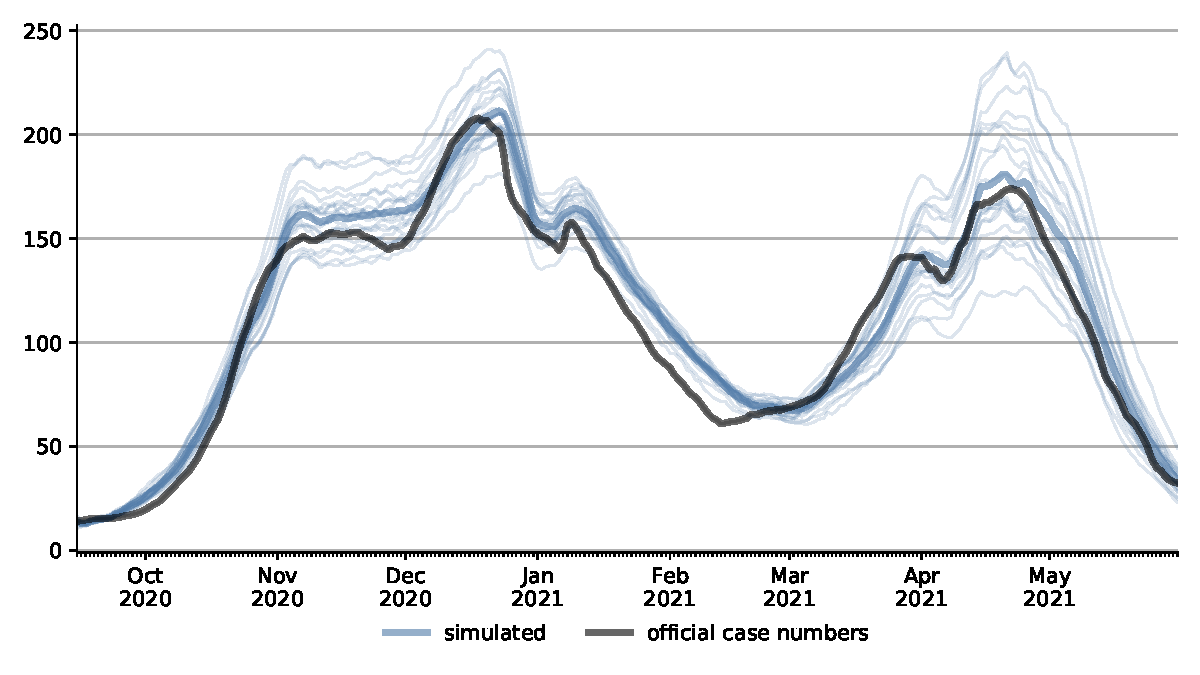
\includegraphics[width=\textwidth]{../figures/results/figures/scenario_comparisons/combined_fit/full_new_known_case_with_single_runs}
\caption{Simulated and Empirical Infections}
\figurenotes{The figure shows the weekly incidence rates per 100,000 people for the reported versus the simulated infections rates.}
\label{fig:aggregated_fit2}
\end{figure}



\begin{figure}[ht]
\centering
  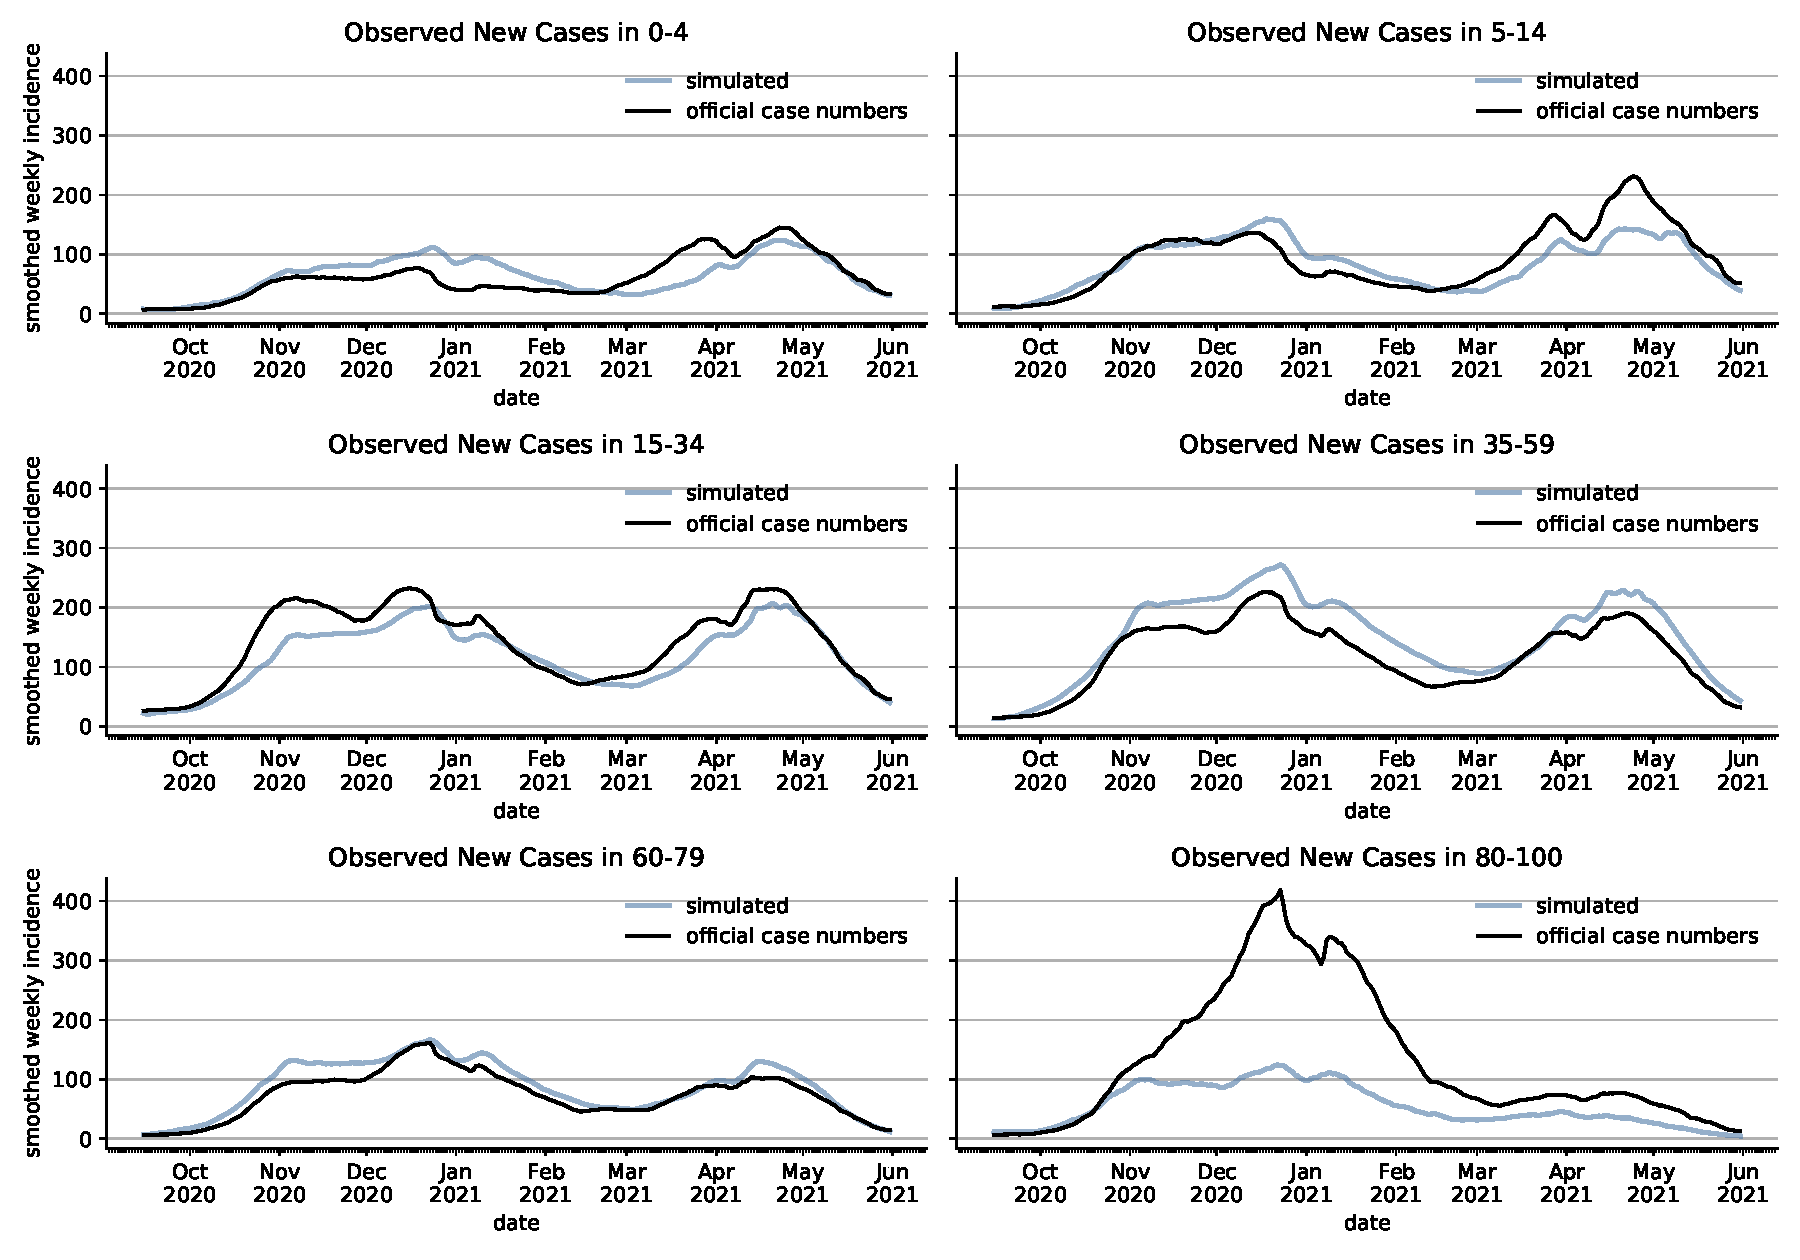
\includegraphics[width=\textwidth]{../figures/results/figures/incidences_by_group/age_group_rki/full_combined_baseline_new_known_case}
\caption{Simulated and Empirical Infections by Age Group}
\figurenotes{The figure shows the weekly incidence rates per 100,000 people for the reported versus the simulated infections rates for different age groups.}
\label{fig:age_group_fit}
\end{figure}


\begin{figure}[ht]
\centering
  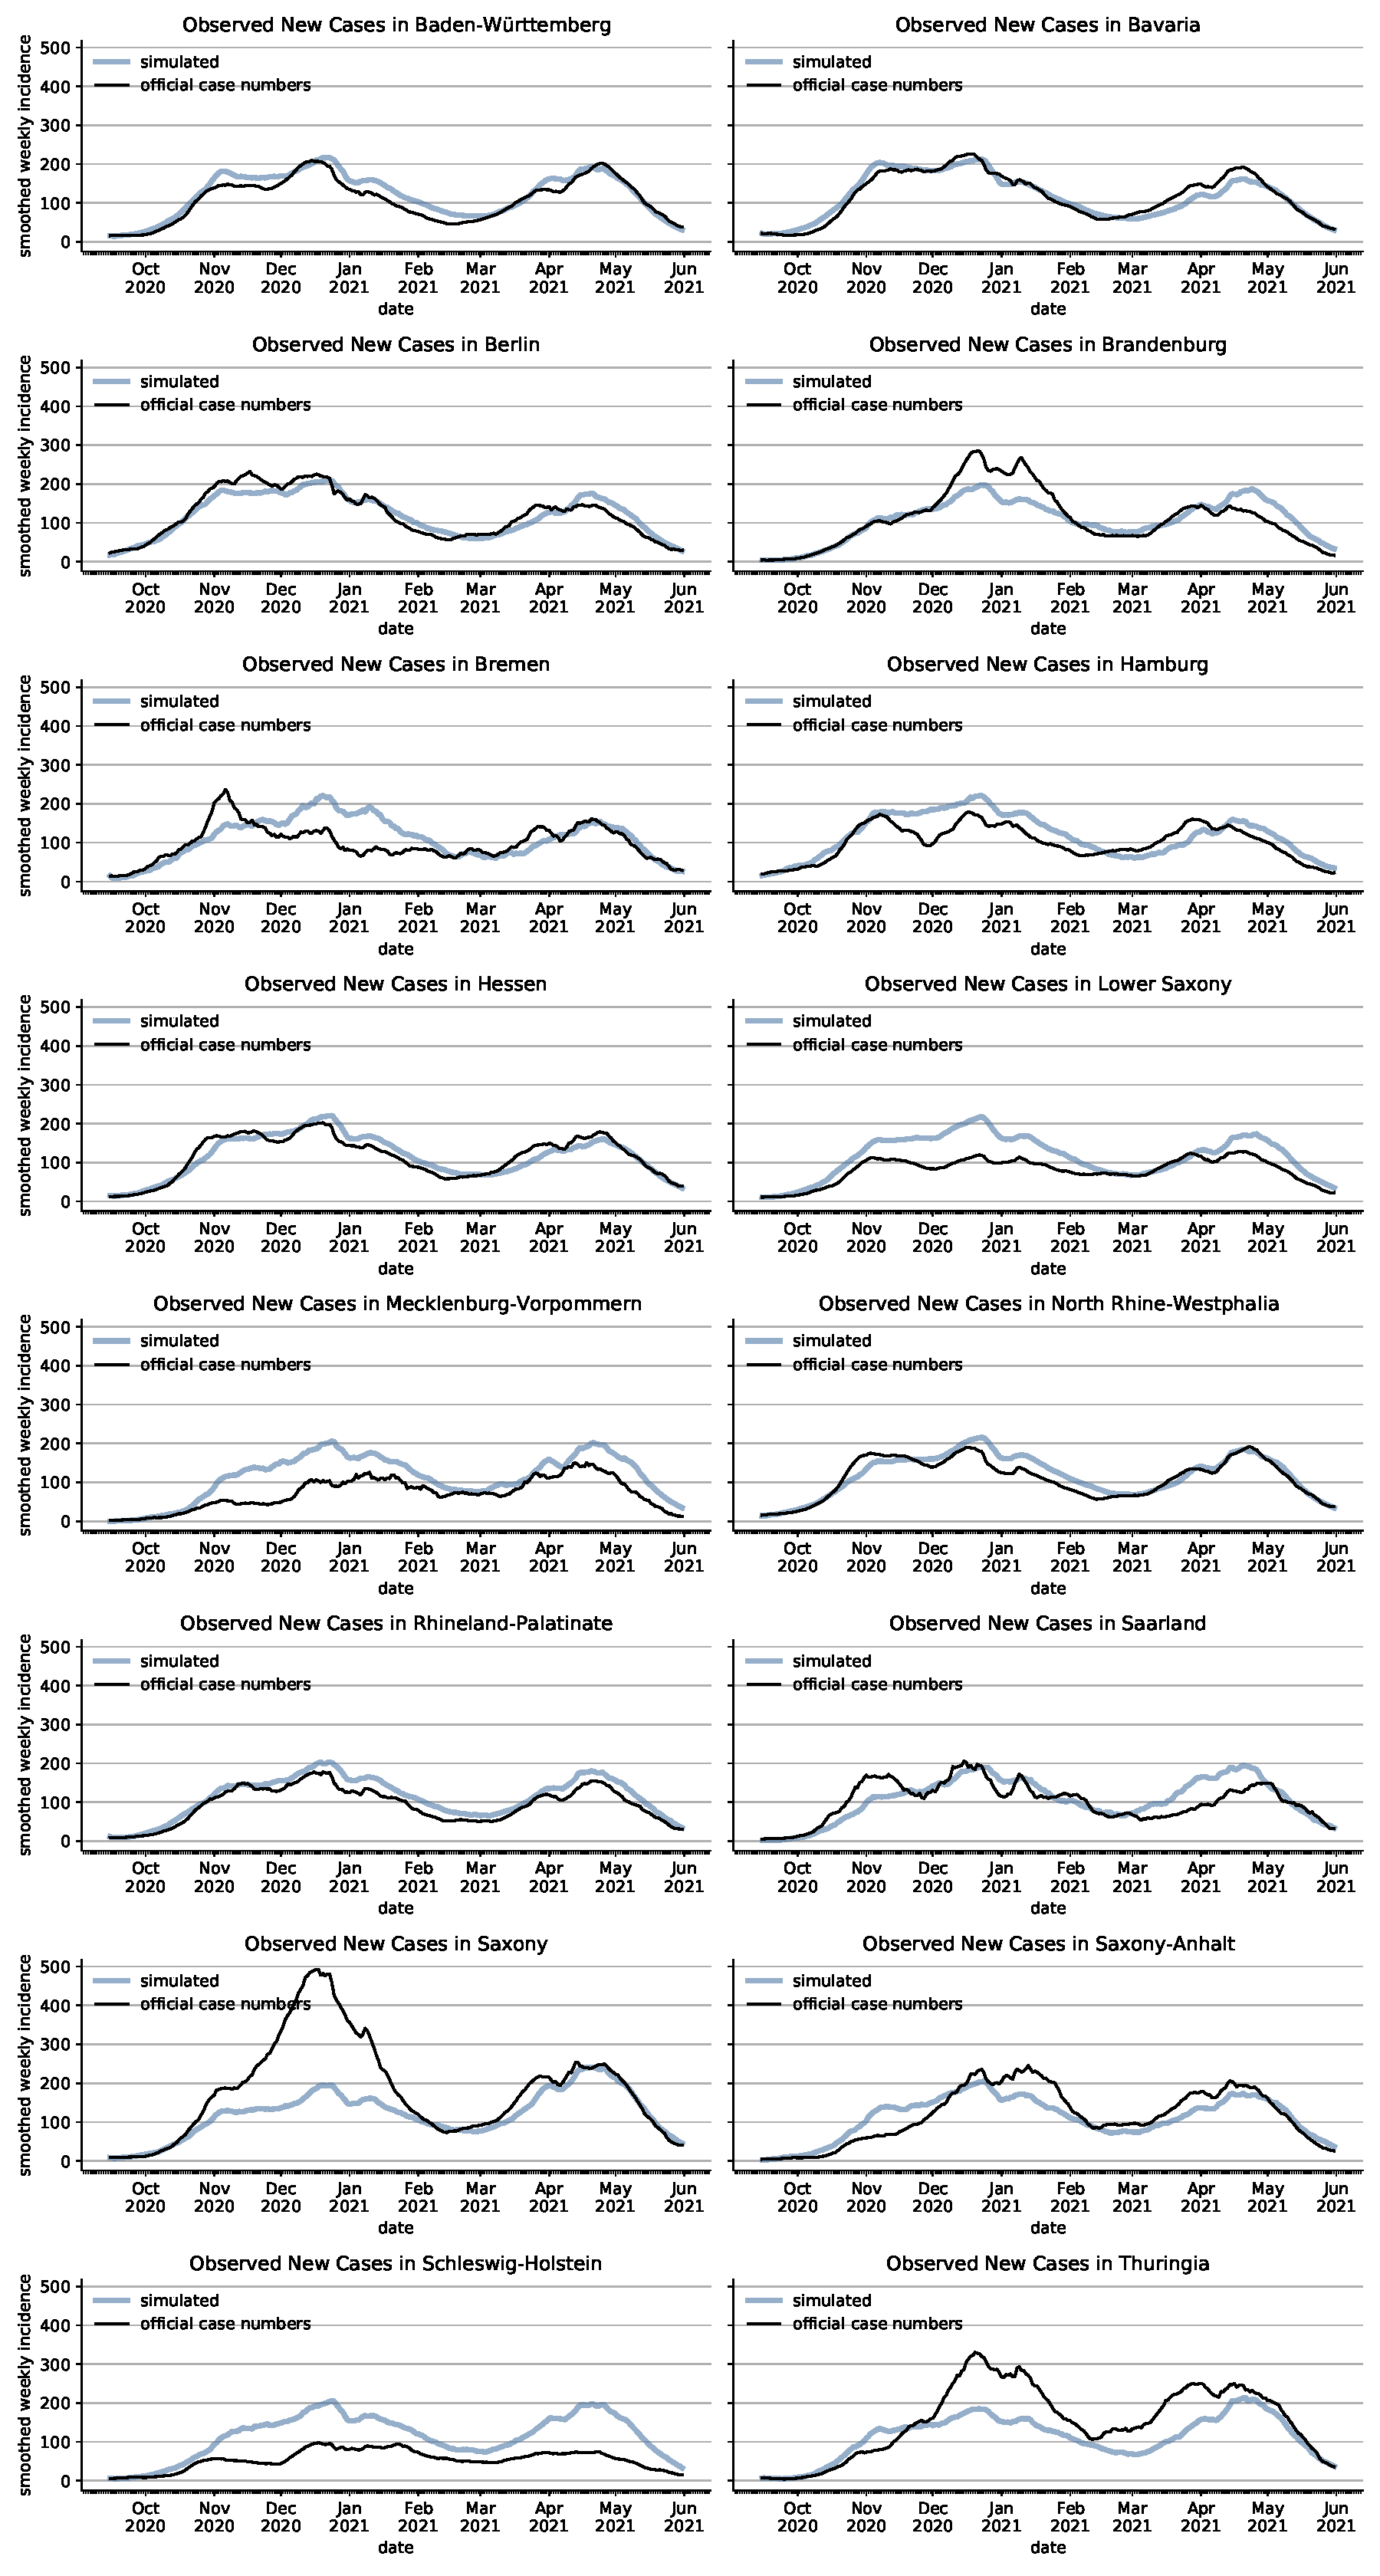
\includegraphics[width=\textwidth]{../figures/results/figures/incidences_by_group/state/full_combined_baseline_new_known_case}
\caption{Simulated and Empirical Infections by Federal State}
\figurenotes{The figure shows the weekly incidence rates per 100,000 people for the reported versus the simulated infections rates for different federal states.}
\label{fig:state_fit}
\end{figure}



\FloatBarrier


\subsection{Scenarios}
\label{subsec:appendix_scenarios}

This is the results section.

\textcolor{red}{The results can be found in `figures/results`. This includes both figures
and tables for lookup of numbers and summary tables.}


\begin{figure}[ht]
\centering
\begin{subfigure}{.6\textwidth}
  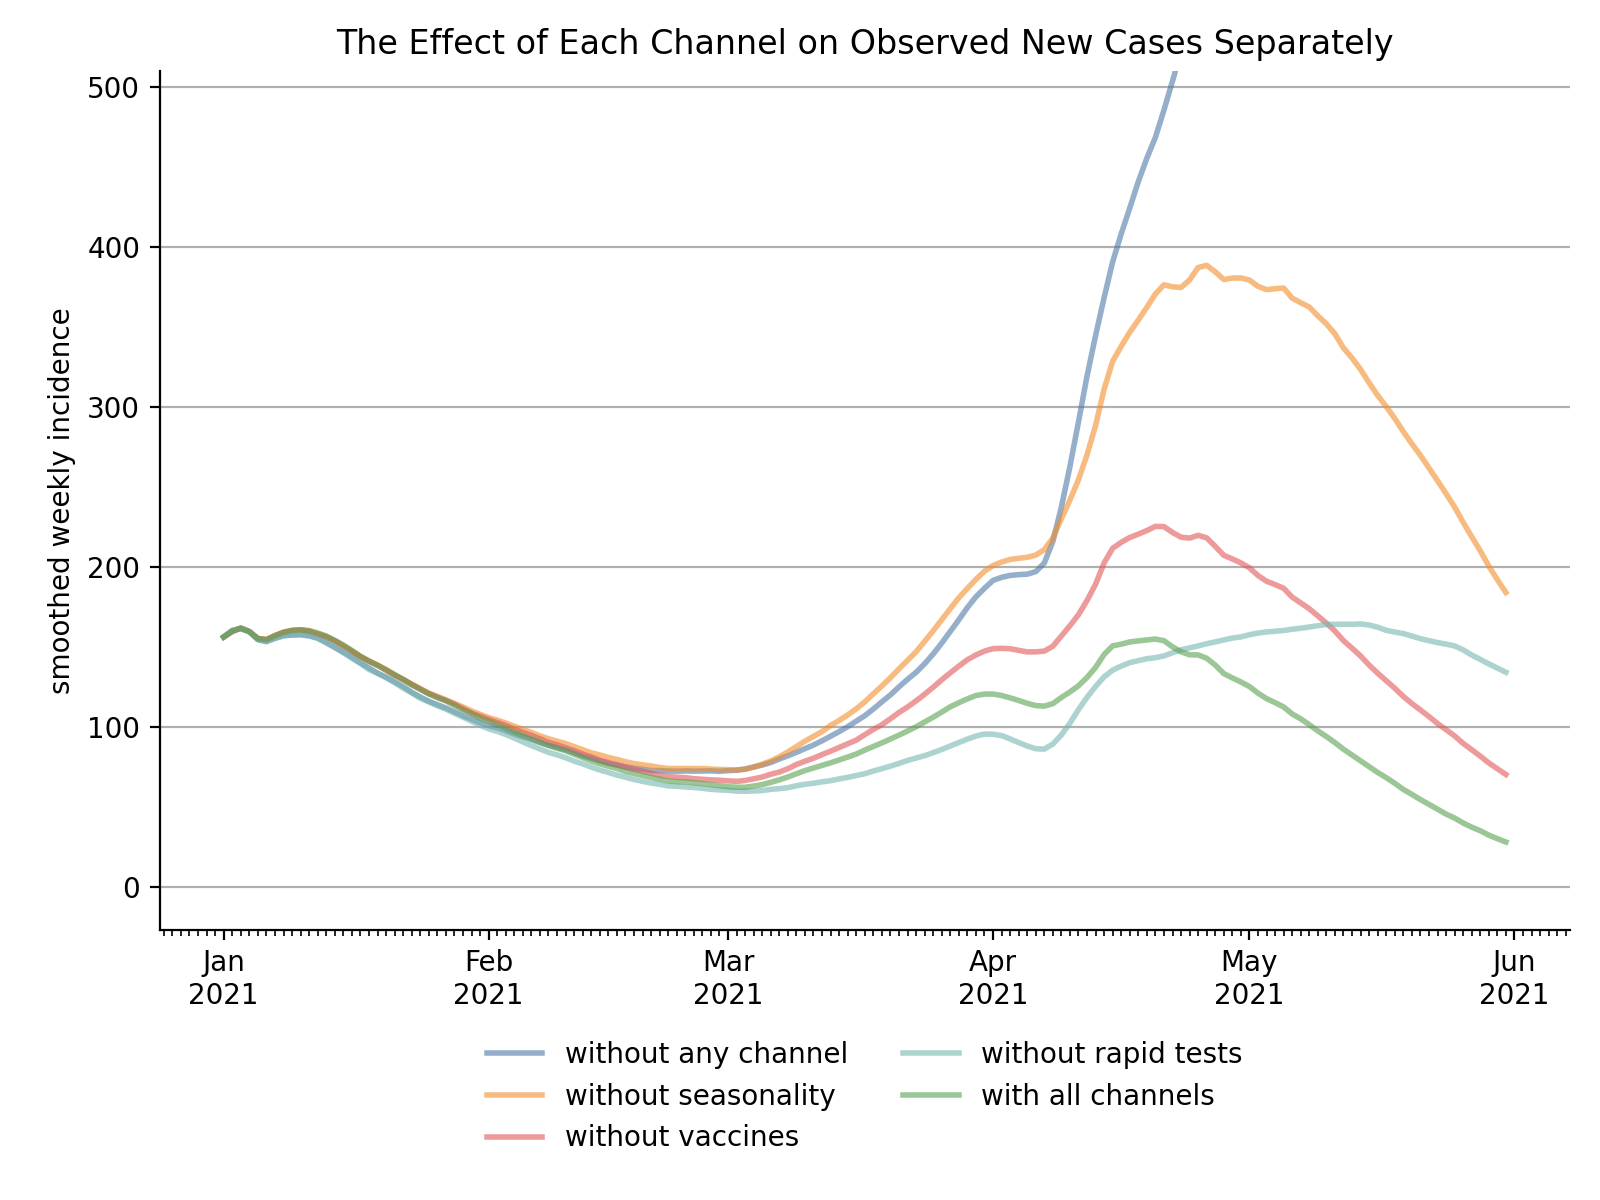
\includegraphics[width=0.9 \textwidth]{../figures/results/figures/scenario_comparisons/one_off_and_combined/full_new_known_case_cropped}
\end{subfigure}%
\begin{subfigure}{.6\textwidth}
  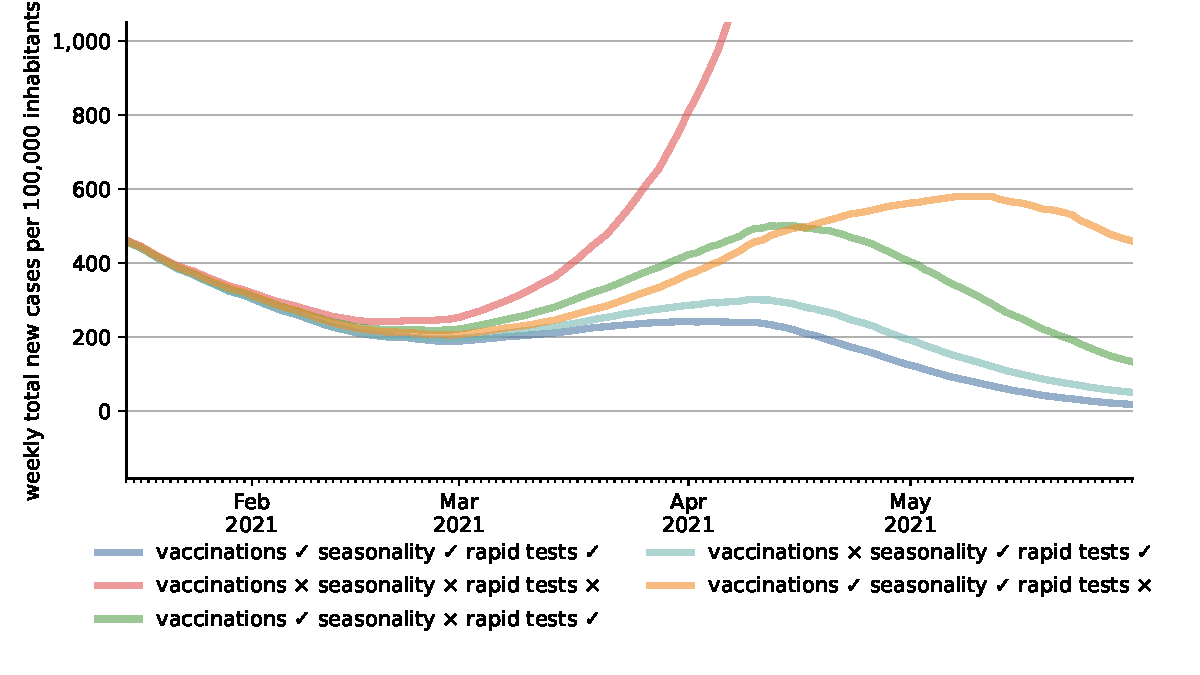
\includegraphics[width=0.9 \textwidth]{../figures/results/figures/scenario_comparisons/one_off_and_combined/full_newly_infected_cropped}
\end{subfigure}
\caption{The Effect of Policies on Observed and Unobserved Cases}
\label{fig:explain_decline}
\figurenotes{\textcolor{red}{\ldots}}
\end{figure}



\begin{figure}[ht]
\centering
\begin{subfigure}{.6\textwidth}
  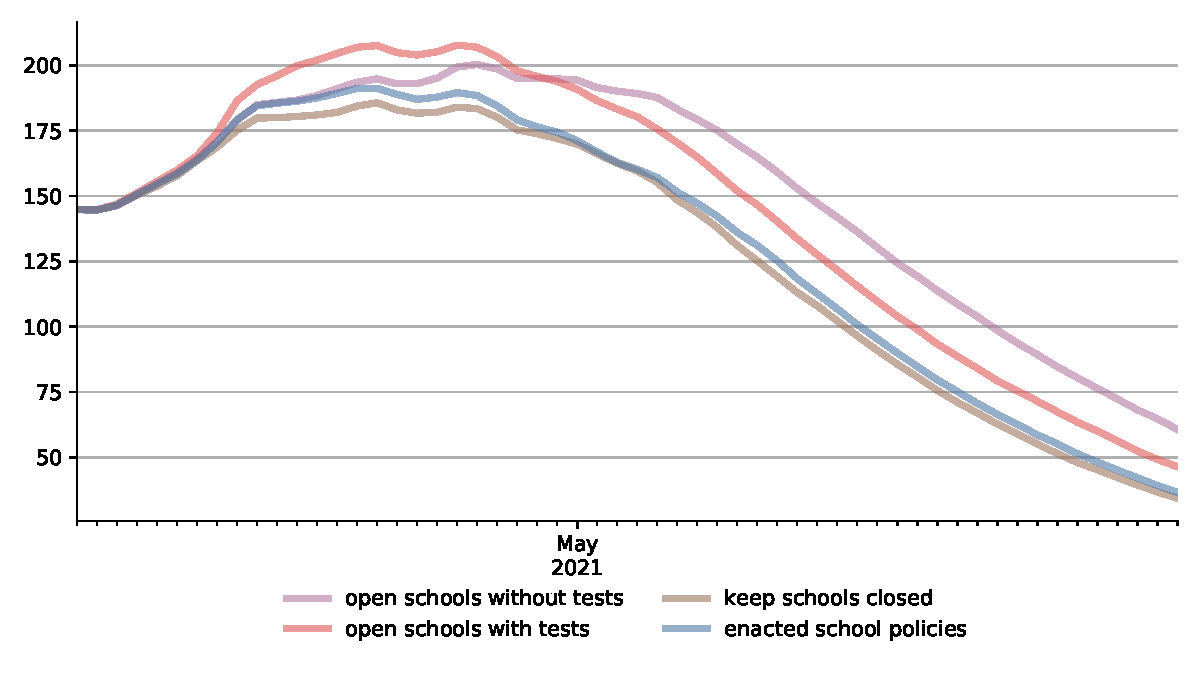
\includegraphics[width=0.9 \textwidth]{../figures/results/figures/scenario_comparisons/school_scenarios/full_new_known_case}
\end{subfigure}%
\begin{subfigure}{.6\textwidth}
  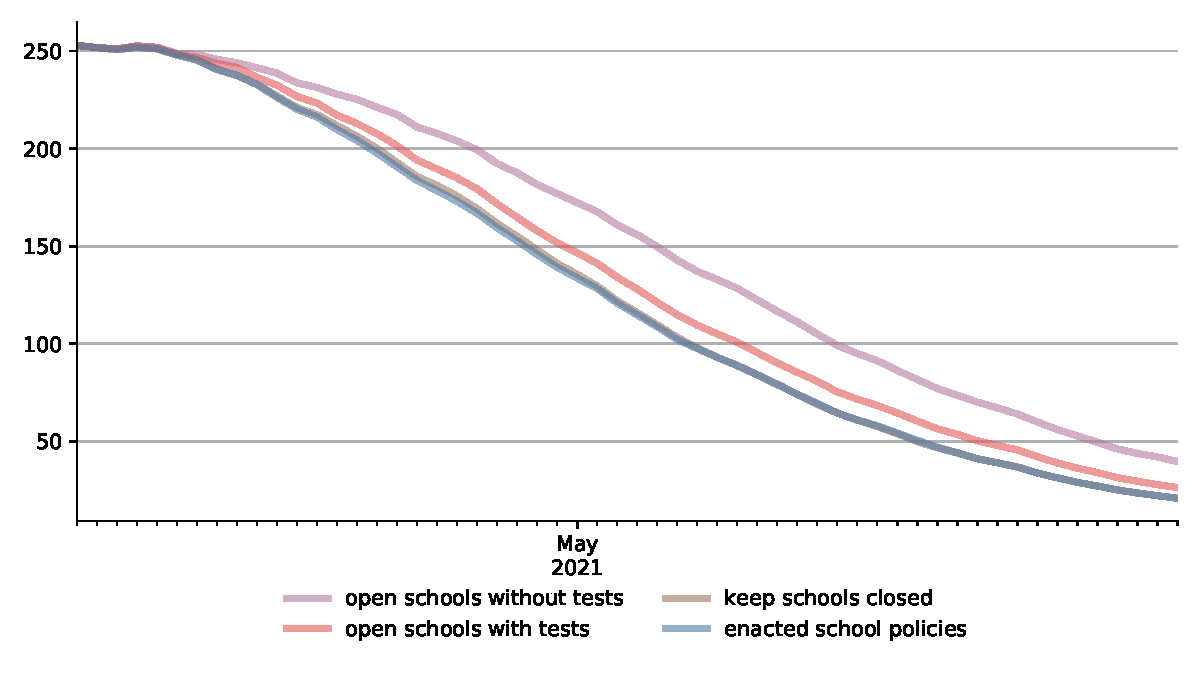
\includegraphics[width=0.9 \textwidth]{../figures/results/figures/scenario_comparisons/school_scenarios/full_newly_infected}
\end{subfigure}
\caption{The Effect of Different School Scenarios on Observed and Unobserved Cases}
\figurenotes{\textcolor{red}{K: One of the scenarios starts too early. Will be fixed with the next full simulations run.}}
\label{fig:school_scenarios}
\end{figure}


\FloatBarrier

\begin{tabular}{lr}
\toprule
{} &  predicted total infections among 5-14 year olds from Easter until 2021-05-31 \\
scenario                               &                                                                               \\
\midrule
 educ open after easter  without tests &                                             775324 \\
 educ open after easter  with tests    &                                             604078 \\
 close educ after easter               &                                             469274 \\
 baseline                              &                                             478080 \\
\bottomrule
\end{tabular}


\FloatBarrier
